\chapter{Introduction to Optimization and Evolutionary Computation}

  Genetic algorithms (GAs) are population-based search methods inspired by natural selection and genetics. They maintain a population of candidate solutions encoded as strings, iteratively producing new generations by selecting the fittest individuals, recombining their information, and occasionally introducing random variation. Although stochastic in their operators, GAs are not blind random walks: they retain and exploit historical information about good solutions to generate promising new search points and thereby drive efficient exploration and exploitation of complex spaces.

  This family of methods was developed from foundational work by Holland and colleagues to both model adaptive processes observed in nature and to design artificial systems that embody those mechanisms. A central aim has been robustness—the ability to balance efficiency with reliability across a wide range of problem environments—which makes GAs attractive when redesign costs are high or when problem structure violates common assumptions (e.g., continuity, differentiability, or unimodality). Because they are conceptually simple, widely applicable, and empirically effective in optimization and control, genetic algorithms have become a practical tool across engineering, science, and business domains \cite{goldberg1989genetic}.

  To place genetic algorithms in context, we first give a concise definition of optimization — the class of problems GAs are commonly used to solve.
    We define optimization as the process of finding the best solution from a set of available alternatives. In mathematical terms, an optimization problem can be formulated as:

  \begin{equation}
  \begin{aligned}
  \text{minimize (or maximize)} \quad & f(x) \\
  \text{subject to} \quad & g_i(x) \leq 0, \quad i = 1, 2, \ldots, m \\
  & h_j(x) = 0, \quad j = 1, 2, \ldots, p \\
  & x \in X
  \end{aligned}
  \end{equation}

  where:
  \begin{itemize}
      \item $f(x)$ is the objective function to be optimized
      \item $g_i(x)$ are inequality constraints
      \item $h_j(x)$ are equality constraints
      \item $X$ is the feasible region
  \end{itemize}

    Optimization problems differ by variable types (discrete, continuous, or mixed-integer) and by structural properties such as linearity, convexity, and the number of objectives. 
    Traditional solution methods include gradient-based techniques (e.g., Newton and quasi-Newton methods) for smooth continuous problems, linear programming (Simplex and interior-point methods) for linear models, and discrete methods (branch-and-bound, dynamic programming) for combinatorial problems. 
    However, these traditional methods have limitations when applied to many complex real-world problems. In the following sections we highlight three key challenges where conventional approaches often struggle, and explain how genetic algorithms can help address them.


    The first problem with traditional optimization methods is their tendency to get trapped in local optima.
    In multi-modal landscapes with many peaks and valleys, gradient-based searches can converge to a local 
    optimum rather than the global optimum. This happens because these methods rely on local gradient 
    information to guide the search process. When the search reaches a local optimum, the gradient 
    becomes zero, causing the algorithm to stop progressing. This limitation is particularly 
    problematic in high-dimensional spaces where the number of local optima can grow exponentially.

  \begin{figure}[H]
    \centering
    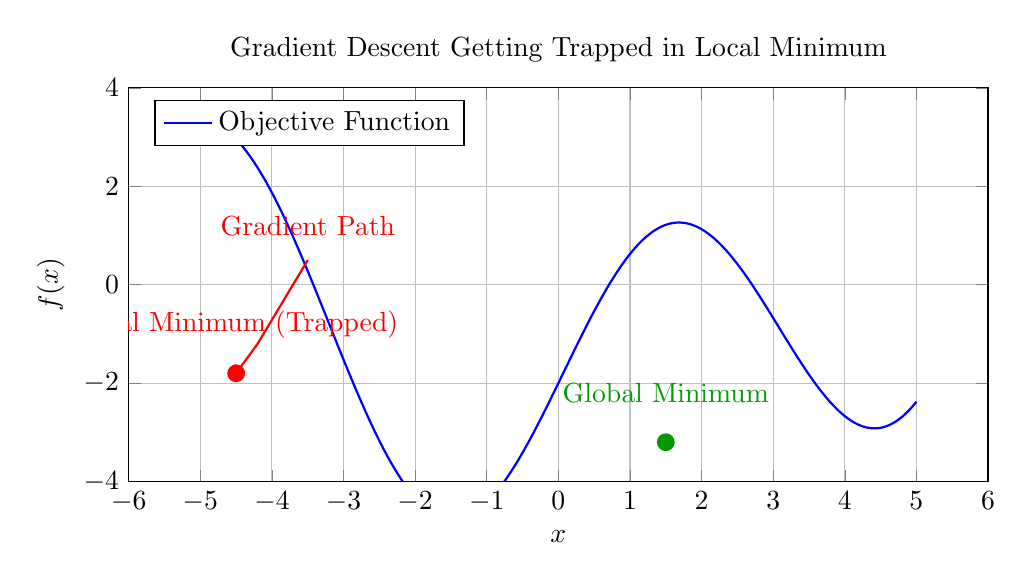
\begin{tikzpicture}
    \begin{axis}[
      width=0.9\textwidth,
      height=5cm,
      scale only axis,
      ymin=-4,
      ymax=4,
      xlabel={$x$},
      ylabel={$f(x)$},
      title={Gradient Descent Getting Trapped in Local Minimum},
      grid=major,
      legend pos=north west,
    ]
    % Multi-modal function
    \addplot[blue, thick, domain=-5:5, samples=200] {sin(deg(x))*3 + 0.1*x^2 - 2};
    \addlegendentry{Objective Function}

    % Local minimum point
    \addplot[red, mark=*, mark size=3pt] coordinates {(-4.5, -1.8)};
    \node[red] at (axis cs:-4.5,-0.8) {Local Minimum (Trapped)};

    % Global minimum point
    \addplot[green!60!black, mark=*, mark size=3pt] coordinates {(1.5, -3.2)};
    \node[green!60!black] at (axis cs:1.5,-2.2) {Global Minimum};

    % Gradient descent path
    \addplot[red, thick, ->] coordinates {(-3.5, 0.5) (-4.2, -1.2) (-4.5, -1.8)};
    \node[red] at (axis cs:-3.5,1.2) {Gradient Path};
    \end{axis}
    \end{tikzpicture}
    \caption{Traditional gradient-based methods follow the local gradient and become trapped in local optima, unable to escape to find the global optimum.}
  \end{figure}

  The second problem with gradient-based methods is that they require the objective function to be differentiable. This becomes a significant limitation when dealing with real-world problems that involve discontinuities, sharp corners, or discrete jumps.
  Such problems are common in engineering design, scheduling, and combinatorial optimization.

  \begin{figure}[H]
  \centering
  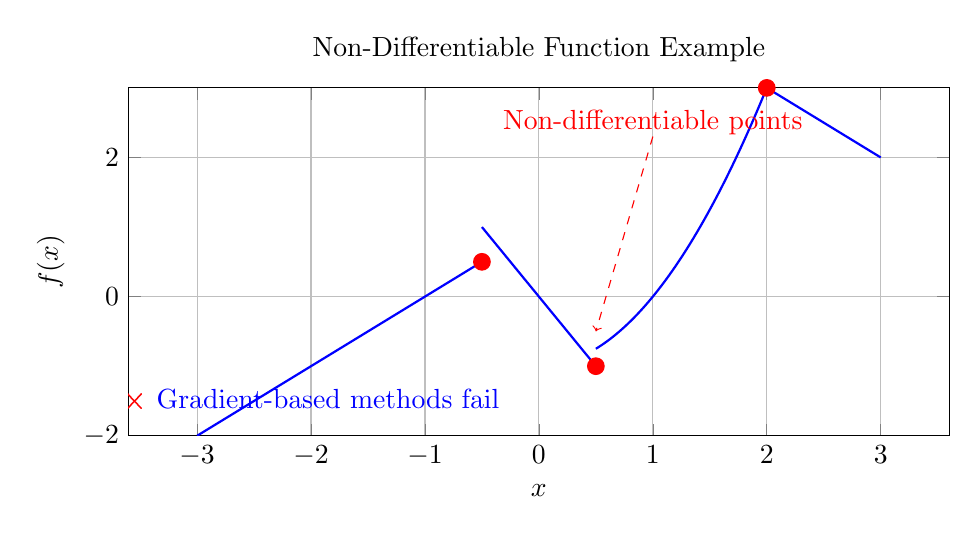
\begin{tikzpicture}
  \begin{axis}[
      width=12cm,
      height=6cm,
      xlabel={$x$},
      ylabel={$f(x)$},
      title={Non-Differentiable Function Example},
      grid=major,
      ymin=-2,
      ymax=3,
  ]
  % Piecewise function with discontinuities
  \addplot[blue, thick, domain=-3:-0.5, samples=50] {x + 1};
  \addplot[blue, thick, domain=-0.5:0.5, samples=50] {-2*x};
  \addplot[blue, thick, domain=0.5:2, samples=50] {x^2 - 1};
  \addplot[blue, thick, domain=2:3, samples=50] {-x + 5};

  % Mark discontinuities
  \addplot[red, mark=*, mark size=3pt, only marks] coordinates {(-0.5, 0.5) (0.5, -1) (2, 3)};
  \node[red] at (axis cs:1, 2.5) {Non-differentiable points};
  \draw[red, dashed, ->] (axis cs:1, 2.3) -- (axis cs:0.5, -0.5);

  \node[blue] at (axis cs:-2, -1.5) {\textcolor{red}{\textbf{×}} Gradient-based methods fail};
  \end{axis}
  \end{tikzpicture}
  \caption{Functions with discontinuities, sharp corners, or discrete jumps cannot be optimized using gradient-based methods.}
  \end{figure}

  % \textbf{How GAs Address This:}
  % \begin{itemize}[leftmargin=*]
  %     \item \textbf{Derivative-free}: GAs only require the ability to evaluate the fitness function, not compute derivatives
  %     \item \textbf{Black-box optimization}: Can handle any function that can be evaluated, regardless of mathematical properties
  %     \item \textbf{Handles discontinuities}: Works equally well with continuous, discrete, or mixed-variable problems
  % \end{itemize}


    While discrete methods such as dynamic programming can handle discontinuities and combinatorial structure, both gradient-based and exact discrete algorithms suffer from the curse of dimensionality: computation typically becomes intractable as problem dimensionality grows.

  \begin{figure}[H]
  \centering
  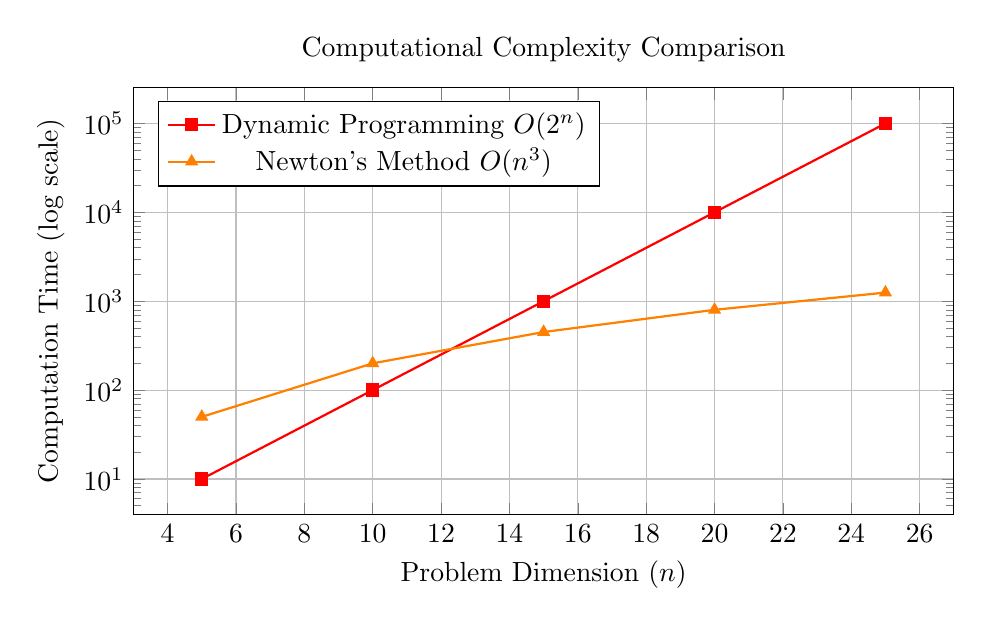
\begin{tikzpicture}
  \begin{axis}[
      width=12cm,
      height=7cm,
      xlabel={Problem Dimension ($n$)},
      ylabel={Computation Time (log scale)},
      title={Computational Complexity Comparison},
      ymode=log,
      legend pos=north west,
      grid=major,
  ]
  % Exponential growth for traditional methods
  \addplot[red, thick, mark=square*] coordinates {
      (5, 10)
      (10, 100)
      (15, 1000)
      (20, 10000)
      (25, 100000)
  };
  \addlegendentry{Dynamic Programming $O(2^n)$}

  % Polynomial growth for Newton
  \addplot[orange, thick, mark=triangle*] coordinates {
      (5, 50)
      (10, 200)
      (15, 450)
      (20, 800)
      (25, 1250)
  };
  \addlegendentry{Newton's Method $O(n^3)$}

  % % Linear-like growth for GA
  % \addplot[green!60!black, thick, mark=*] coordinates {
  %     (5, 20)
  %     (10, 35)
  %     (15, 50)
  %     (20, 65)
  %     (25, 80)
  %     (50, 155)
  %     (100, 305)
  % };
  % \addlegendentry{Genetic Algorithm (approximate)}

  \end{axis}
  \end{tikzpicture}
    \caption{Traditional optimization methods often exhibit exponential or high polynomial growth in computation time as problem dimensionality increases, making them impractical for large-scale problems.}
  \end{figure}

  % \textbf{How GAs Address This:}
  % \begin{itemize}[leftmargin=*]
  %     \item \textbf{Heuristic approach}: Trade optimality guarantee for computational efficiency
  %     \item \textbf{Parallel evaluation}: Population members can be evaluated in parallel
  %     \item \textbf{Scalability}: Computational cost grows more gracefully with problem size
  % \end{itemize}
  %



    Therefore, we can summarize how genetic algorithms effectively address the fundamental limitations of traditional optimization methods in the following table:
  \begin{figure}[H]
  \centering
  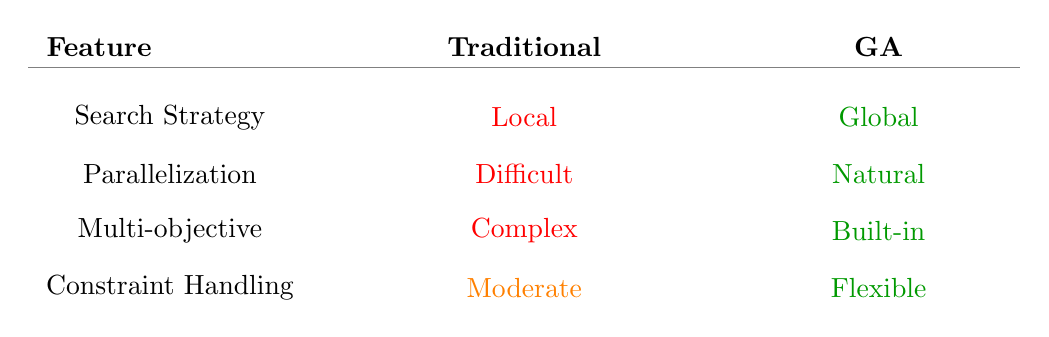
\begin{tikzpicture}[scale=0.9]
      % Comparison rows
      \node[font=\bfseries] at (1, 4) {Feature};
      \node[font=\bfseries] at (7, 4) {Traditional};
      \node[font=\bfseries] at (12, 4) {GA};
      
      \draw[gray] (0, 3.7) -- (14, 3.7);
      
      \node[align=left] at (2, 3) {Search Strategy};
      \node[red] at (7, 3) {Local};
      \node[green!60!black] at (12, 3) {Global};
      
      \node[align=left] at (2, 2.2) {Parallelization};
      \node[red] at (7, 2.2) {Difficult};
      \node[green!60!black] at (12, 2.2) {Natural};
      
      \node[align=left] at (2, 1.4) {Multi-objective};
      \node[red] at (7, 1.4) {Complex};
      \node[green!60!black] at (12, 1.4) {Built-in};
      
      \node[align=left] at (2, 0.6) {Constraint Handling};
      \node[orange] at (7, 0.6) {Moderate};
      \node[green!60!black] at (12, 0.6) {Flexible};
  \end{tikzpicture}
  \caption{Comprehensive comparison showing how GAs address the fundamental limitations of traditional optimization methods.}
  \end{figure}

  \section{Introduction to Evolutionary Computation}
  Evolutionary computation is a family of algorithms inspired by biological evolution~\cite{holland1975adaptation, eiben2015introduction}. These algorithms use mechanisms such as selection, which implements the principle of survival of the fittest, reproduction for creating offspring, mutation to introduce random changes, and crossover for combining genetic material from different individuals.

  \subsection{Advantages of Evolutionary Approaches}
  Evolutionary approaches offer several compelling advantages that make them attractive for complex optimization problems. They require no gradient information, which is particularly valuable when dealing with black-box optimization scenarios. These algorithms can effectively handle discontinuous, noisy, and multi-modal functions that would challenge traditional optimization methods. Their versatility extends to both continuous and discrete optimization problems, making them applicable across diverse domains. The population-based search strategy provides inherent robustness against local optima, and when properly configured, these algorithms can find global optima in challenging search spaces.

  \subsection{Types of Evolutionary Algorithms}
  The field of evolutionary computation encompasses several distinct algorithmic families, each with its own characteristics and strengths. Genetic Algorithms (GA) are inspired by natural selection and were among the first evolutionary approaches developed~\cite{holland1975adaptation, goldberg1989genetic}. Evolution Strategies (ES) focus specifically on real-valued optimization problems and have proven particularly effective in continuous domains~\cite{back1996evolutionary}. Evolutionary Programming (EP) places emphasis on behavioral evolution rather than genetic representations~\cite{fogel1995evolutionary, fogel2006evolutionary}. Finally, Genetic Programming (GP) extends evolutionary principles to the evolution of computer programs themselves, enabling the automatic generation of code~\cite{koza1992genetic}.

  \subsection{Applications of Evolutionary Computation}
  Evolutionary algorithms have demonstrated remarkable success across a wide range of practical applications~\cite{gen2007genetic, sivanandam2008introduction, eiben2015introduction}. In engineering design optimization, they have been used to find optimal configurations for complex systems~\cite{yildiz2023novel}. The field of machine learning has benefited from evolutionary approaches, particularly in neural network training where they can optimize both architectures and weights~\cite{montana1989training, murad2025hybrid}. Scheduling and timetabling problems, which are notoriously difficult combinatorial optimization challenges, have been successfully addressed using evolutionary methods~\cite{gu2022hybrid, fajrin2020multi}. Beyond these areas, evolutionary algorithms have found applications in financial modeling, bioinformatics, and game playing strategy development, demonstrating their versatility across diverse problem domains.


  \subsection{Simple Examples of Genetic Algorithm Applications}

  Genetic Algorithms possess an extraordinary capability in finding optimal solutions for problems with vast search spaces.

  \subsection{Maximizing a Quadratic Function}
  A classic example often used to illustrate how Genetic Algorithms work is the problem of maximizing a simple quadratic function, such as $f(x) = x^2$ in the range $0 \leq x \leq 31$. In this case, the optimal solution is clear: $x = 31$, yielding $f(x) = 961$. However, this problem is used to demonstrate how Genetic Algorithms, despite starting with a random population (for example, four 5-bit binary chromosomes), can gradually combine features (building blocks) from existing solutions to achieve better results.

  Through cycles of selection, crossover, and mutation, Genetic Algorithms show how both the maximum and average performance of the population increases from one generation to the next. Within a few generations, individuals representing $x = 31$ (binary 11111) will dominate the population.

  \begin{figure}[h]
  \centering
  \includegraphics[width=0.7\textwidth]{figures/buku_ajar_page_4.png}
  \caption{Illustration of GA cycle and variations}
  \label{fig:ga_intro_cycle}
  \end{figure}

  \subsection{Travelling Salesman Problem}
  Another example of genetic algorithm application is the Travelling Salesman Problem (TSP), where Genetic Algorithms are used to find the shortest route visiting a number of cities—a highly complex combinatorial optimization problem.


    % Note: the detailed, domain-specific examples that previously followed (scheduling, network design, VLSI) were removed here to avoid repetition with the earlier "Applications" section. Key examples remain in the "Applications of Evolutionary Computation" section above.

  \section{Genetic Algorithm Flow}

  Genetic algorithms maintain a population of individuals, denoted as $P(t)$ for generation $t$, where each individual represents a potential solution to the problem at hand. This cycle runs iteratively through steps that mimic the evolution process.

  After the initial population $P(0)$ is initialized and its fitness evaluated, the selection process begins, where fitter individuals are probabilistically selected to enter the mating pool. Selected individuals then undergo stochastic transformation through genetic operators. The crossover operator is responsible for exploiting the best information from parents, while mutation is tasked with exploring the search space by introducing new genetic material.

  Newly generated individuals, called offspring $C(t)$, are then evaluated for their fitness. A new population $P(t+1)$ is formed by selecting fitter individuals from both the parent and offspring populations through a replacement scheme. This process is repeated for several generations until the algorithm converges, pointing to the best individual, which is expected to represent an optimal or suboptimal solution to the problem.

  \section{Genetic Algorithm Variations}

  Although the Simple Generational Genetic Algorithm serves as the basic framework, various modifications have been developed to improve performance in dealing with problem complexity. Some of these modifications include:

  \subsection{Hybrid GA}
  Hybrid GA (HGA) combines Genetic Algorithms with conventional local search techniques~\cite{majhi2025novel, murad2025hybrid}. In a hybrid approach, Genetic Algorithms perform global exploration across the population, while local search is used for refinement around promising solutions. This approach often outperforms single methods because it leverages the complementary advantages of both search techniques.

  \subsection{Adaptive GA}
  Adaptive GA (AGA) is a Genetic Algorithm where strategic parameters (such as crossover or mutation probabilities) are dynamically adjusted during the evolution process, often using feedback from population performance to balance exploitation and exploration effectively~\cite{shams2025resolving, srinivas1994genetic}.

  \subsection{Parallel GA}
  Parallel Genetic Algorithms divide the population into different sub-populations across various processors, allowing periodic information exchange (migration) to increase diversity and convergence speed.

  \section{Chapter Summary}
  This chapter introduced the fundamental concepts of optimization and evolutionary computation. We explored the limitations of traditional optimization methods and highlighted the advantages of evolutionary approaches. We also examined specific examples of GA applications including function optimization, TSP, scheduling, network design, and VLSI design. The GA flow and various modifications were discussed to provide a comprehensive understanding of genetic algorithms.

  \section{Key Concepts}
  \begin{itemize}
      \item Optimization problem formulation
      \item Objective functions and constraints
      \item Local vs. global optima
      \item Evolutionary computation principles
      \item Population-based search
  \end{itemize}

  \section{Further Reading}
  \begin{itemize}
      \item Deb, K. (2001). Multi-objective optimization using evolutionary algorithms.
      \item Eiben, A. E., \& Smith, J. E. (2015). Introduction to evolutionary computing.
      \item Goldberg, D. E. (1989). Genetic algorithms in search, optimization, and machine learning.
  \end{itemize}
